\documentclass[11pt,a4paper]{article}
\usepackage[T1]{fontenc}
\usepackage[utf8]{inputenc}
\usepackage[polish]{babel}
\usepackage{amsmath}
\usepackage{amsfonts}
\usepackage{graphicx}
\usepackage[margin=0.7in]{geometry}
\author{Kamil Kuczaj}
\title{Sprawozdanie z Laboratorium 8 - Pomiar czasu algorytmów BFS i DFS grafu nieskierowanego.}
\date{\today}
\begin{document}

\maketitle

\section{Wstęp}
\hspace{4ex}Zadaniem na laboratorium był pomiar czasu przeszukania grafu korzystając z dwóch algorytmów:
\begin{enumerate}
\item DFS (\textit{Depth First Search}, czyli tzw. przeszukiwanie wgłąb grafu
\item BFS (\textit{Breadth First Search}, czyli tzw. przeszukiwanie wszerz grafu.
\end{enumerate} Wg teorii oba algorytmy mają złożoność obliczeniową równą O(E), gdzie E jest liczbą krawędzi w grafie (\textit{ang. Edge}. Zdecydowano się na implementację grafu na postawie listy sąsiedztwa. Jest to trudniejsza konstrukcja, jednak oba algorytmy będą szybsze na takiej strukturze. Iterowanie po liście jest znacznie szybsze niż iterowanie po tablicy oraz pozwala zaoszczędzić wiele pamięci operacyjnej.\\\\W naszym przypadku mieliśmy załadować kolejno $10^1$, $10^3$, $10^5$, $10^6$ oraz sprawdzić czas wyszukiwania znanego elementu. Sposób generacji polegał na tym, aby stworzyć \textit{n} wierzchołków, połączyć każdy wierzchołek z następnym krawędzią o wadze równej 1. Łącząc ostatni wierzchołek z pierwszym powstawało koło. Następnie $round(ln(n))$ pierwszych wierzchołków pseudolosowo (biblioteka \textit{<cstdlib>}) było łączone krawędzią o wadze 1 z $round(ln(n))$ innymi wierzchołkami. W ten sposób można było otrzymać:

\begin{table}[htbp]
\caption{}
\begin{center}
\begin{tabular}{|c|c|c|c|c|c|}
\hline
\textbf{n} & \textbf{10} & \textbf{100} & \textbf{1000} & \textbf{10000} & \textbf{100000} \\ \hline
\textbf{round( ln(n) )} & 2 & 5 & 7 & 9 & 12 \\ \hline
\textbf{V + E = n + ln(n)*ln(n)} & 14 & 125 & 1049 & 10081 & 100144 \\ \hline
\end{tabular}
\end{center}
\label{zlozonosc}
\end{table}

\newpage

\section{Specyfikacja komputera}

\begin{table}[htbp]
\caption{}
\begin{center}
	\begin{tabular}{| r | c |}
	\hline
	Wersja kompilatora \textit{g++} & 4.8.4 \\ \hline
	System & Ubuntu 14.04.4 \\ \hline
	Procesor	 & Intel Core i5 2510M 2.3 GHz \\ \hline
	Pamięć RAM & 8 GB DDR3 1600 MHz \\ \hline
	Dysk twardy & HDD (5400 obr./min) \\ \hline
	Rozmiar zmiennej \textit{int} & 4 bajty \\ \hline
	\end{tabular}
\end{center}
\label{specyfikacja}
\end{table}

\section{Pomiary oraz ich interpretacja}


\begin{figure}[htbp]
\begin{center}
	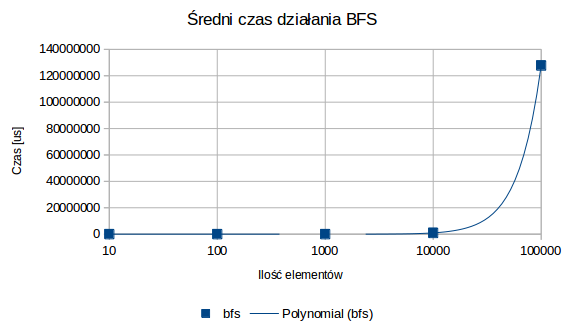
\includegraphics[scale=0.7]{../wyniki/BFS.png}
\end{center}
\caption{Wyniki wraz z regresją kwadratową. Oś odciętych w skali logarytmicznej.}
\end{figure}


\begin{table}[htbp]
\caption{}
\begin{center}
\begin{tabular}{|c|c|c|c|c|c|}
\hline
\textbf{Ilość elementów} & \textbf{10} & \textbf{100} & \textbf{1 000} & \textbf{10 000} & \textbf{100 000} \\ \hline
\textbf{Średni czas BFS [us]} & 18,3 & 170,76 & 10464,54 & 961902,28 & 127787700 \\ \hline
\textbf{Średni czas BFS [s]} & 0,0000183 & 0,00017076 & 0,01046454 & 0,96190228 & 127,7877 \\ \hline
\end{tabular}
\end{center}
\label{bfs_sredni}
\end{table}



\begin{table}[htbp]
\caption{}
\begin{center}
\begin{tabular}{|c|c|c|c|c|c|}
\hline
\textbf{} & \multicolumn{ 5}{c|}{\textbf{BFS (czasy w mikrosekundach)}} \\ \hline
\textbf{Ilość elementów} & \textbf{10} & \textbf{100} & \textbf{1 000} & \textbf{10 000} & \textbf{100 000} \\ \hline
\textbf{Pomiar nr 1} & 20 & 170 & 10 683 & 926 741 & 125 348 000 \\ \hline
\textbf{Pomiar nr 2} & 21 & 170 & 9 971 & 961 815 & 138 205 000 \\ \hline
\textbf{Pomiar nr 3} & 18 & 168 & 10 918 & 927 253 & 122 429 000 \\ \hline
\textbf{Pomiar nr 4} & 17 & 170 & 11 563 & 935 551 & 133 909 000 \\ \hline
\textbf{Pomiar nr 5} & 16 & 170 & 10 186 & 928 440 & 124 432 000 \\ \hline
\textbf{Pomiar nr 6} & 21 & 171 & 12 834 & 930 681 & 132 298 000 \\ \hline
\textbf{Pomiar nr 7} & 17 & 167 & 10 637 & 931 452 & 119 586 000 \\ \hline
\textbf{Pomiar nr 8} & 17 & 166 & 9 990 & 945 340 & 131 274 000 \\ \hline
\textbf{Pomiar nr 9} & 15 & 178 & 10 174 & 960 872 & 119 598 000 \\ \hline
\textbf{Pomiar nr 10} & 15 & 169 & 10 132 & 931 477 & 130 798 000 \\ \hline
\textbf{Pomiar nr 11} & 16 & 168 & 10 033 & 946 035 &  \\ \hline
\textbf{Pomiar nr 12} & 16 & 165 & 10 009 & 950 542 &  \\ \hline
\textbf{Pomiar nr 13} & 16 & 170 & 11 172 & 964 619 &  \\ \hline
\textbf{Pomiar nr 14} & 16 & 171 & 11 589 & 935 598 &  \\ \hline
\textbf{Pomiar nr 15} & 15 & 169 & 10 965 & 935 523 &  \\ \hline
\textbf{Pomiar nr 16} & 15 & 168 & 11 419 & 943 430 &  \\ \hline
\textbf{Pomiar nr 17} & 16 & 178 & 12 129 & 926 995 &  \\ \hline
\textbf{Pomiar nr 18} & 16 & 177 & 11 021 & 975 528 &  \\ \hline
\textbf{Pomiar nr 19} & 15 & 179 & 10 682 & 937 638 &  \\ \hline
\textbf{Pomiar nr 20} & 16 & 167 & 11 351 & 933 311 &  \\ \hline
\textbf{Pomiar nr 21} & 15 & 167 & 10 938 & 926 383 &  \\ \hline
\textbf{Pomiar nr 22} & 15 & 167 & 11 065 & 932 908 &  \\ \hline
\textbf{Pomiar nr 23} & 17 & 167 & 10 409 & 929 015 &  \\ \hline
\textbf{Pomiar nr 24} & 26 & 166 & 10 391 & 936 482 &  \\ \hline
\textbf{Pomiar nr 25} & 18 & 167 & 9 927 & 931 784 &  \\ \hline
\textbf{Pomiar nr 26} & 25 & 169 & 10 060 & 931 614 &  \\ \hline
\textbf{Pomiar nr 27} & 25 & 167 & 10 068 & 925 970 &  \\ \hline
\textbf{Pomiar nr 28} & 35 & 169 & 9 892 & 931 366 &  \\ \hline
\textbf{Pomiar nr 29} & 25 & 166 & 9 971 & 927 612 &  \\ \hline
\textbf{Pomiar nr 30} & 25 & 168 & 10 527 & 931 082 &  \\ \hline
\textbf{Pomiar nr 31} & 25 & 166 & 9 748 & 926 937 &  \\ \hline
\textbf{Pomiar nr 32} & 25 & 169 & 10 109 & 933 378 &  \\ \hline
\textbf{Pomiar nr 33} & 24 & 167 & 10 667 & 999 666 &  \\ \hline
\textbf{Pomiar nr 34} & 22 & 168 & 10 087 & 936 703 &  \\ \hline
\textbf{Pomiar nr 35} & 17 & 169 & 10 089 & 932 640 &  \\ \hline
\textbf{Pomiar nr 36} & 17 & 167 & 10 171 & 939 062 &  \\ \hline
\textbf{Pomiar nr 37} & 17 & 168 & 9 727 & 1 011 730 &  \\ \hline
\textbf{Pomiar nr 38} & 16 & 175 & 10 862 & 1 174 270 &  \\ \hline
\textbf{Pomiar nr 39} & 17 & 167 & 10 084 & 1 086 720 &  \\ \hline
\end{tabular}
\end{center}
\label{bfs1}
\end{table}


\begin{center}
\begin{tabular}{|c|c|c|c|c|c|}
\hline
\textbf{} & \multicolumn{ 5}{c|}{\textbf{BFS (czasy w mikrosekundach)}} \\ \hline
\textbf{Ilość elementów} & \textbf{10} & \textbf{100} & \textbf{1 000} & \textbf{10 000} & \textbf{100 000} \\ \hline
\textbf{Pomiar nr 40} & 15 & 169 & 9 667 & 1 009 240 &  \\ \hline
\textbf{Pomiar nr 41} & 16 & 167 & 9 849 & 956 614 &  \\ \hline
\textbf{Pomiar nr 42} & 16 & 168 & 10 844 & 938 082 &  \\ \hline
\textbf{Pomiar nr 43} & 16 & 167 & 9 822 & 958 697 &  \\ \hline
\textbf{Pomiar nr 44} & 16 & 168 & 10 024 & 966 607 &  \\ \hline
\textbf{Pomiar nr 45} & 16 & 167 & 10 531 & 954 374 &  \\ \hline
\textbf{Pomiar nr 46} & 16 & 166 & 9 982 & 943 325 &  \\ \hline
\textbf{Pomiar nr 47} & 16 & 165 & 10 108 & 999 292 &  \\ \hline
\textbf{Pomiar nr 48} & 16 & 180 & 10 377 & 1 184 950 &  \\ \hline
\textbf{Pomiar nr 49} & 16 & 204 & 9 678 & 1 095 680 &  \\ \hline
\textbf{Pomiar nr 50} & 16 & 217 & 10 095 & 1 014 090 &  \\ \hline
\end{tabular}
\label{bfs2}
\end{center}




\begin{figure}[htbp]
\begin{center}
	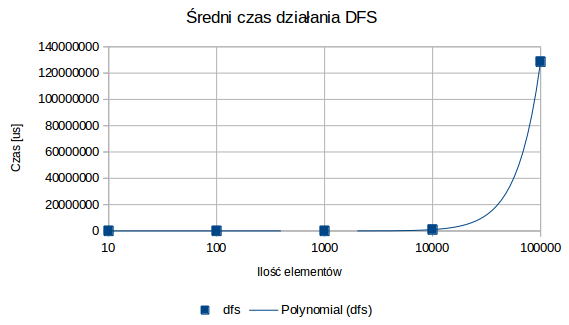
\includegraphics[scale=0.7]{../wyniki/DFS.png}
\end{center}
\caption{Wyniki wraz z regresją kwadratową. Oś odciętych w skali logarytmicznej.}
\end{figure}



\begin{table}[htbp]
\caption{}
\begin{center}
\begin{tabular}{|c|c|c|c|c|c|}
\hline
\textbf{Ilość elementów} & \textbf{10} & \textbf{100} & \textbf{1 000} & \textbf{10 000} & \textbf{100 000} \\ \hline
\textbf{Średni czas DFS [us]} & 15,22 & 210,96 & 11246,56 & 1010026,8 & 128707900 \\ \hline
\textbf{Średni czas DFS [s]} & 0,00001522 & 0,00021096 & 0,01124656 & 1,0100268 & 128,7079 \\ \hline
\end{tabular}
\end{center}
\label{dfs_sredni}
\end{table}



\begin{table}[htbp]
\caption{}
\begin{center}
\begin{tabular}{|c|c|c|c|c|c|}
\hline
\textbf{} & \multicolumn{ 5}{c|}{\textbf{DFS (czasy w mikrosekundach)}} \\ \hline
\textbf{Ilość elementów} & \textbf{10} & \textbf{100} & \textbf{1 000} & \textbf{10 000} & \textbf{100 000} \\ \hline
\textbf{Pomiar nr 1} & 15 & 236 & 11 123 & 977 594 & 123 924 000 \\ \hline
\textbf{Pomiar nr 2} & 14 & 232 & 11 055 & 1 036 480 & 134 461 000 \\ \hline
\textbf{Pomiar nr 3} & 25 & 222 & 10 931 & 981 043 & 122 972 000 \\ \hline
\textbf{Pomiar nr 4} & 13 & 334 & 10 373 & 974 835 & 133 993 000 \\ \hline
\textbf{Pomiar nr 5} & 11 & 183 & 11 018 & 981 799 & 123 124 000 \\ \hline
\textbf{Pomiar nr 6} & 11 & 188 & 11 233 & 980 246 & 134 154 000 \\ \hline
\textbf{Pomiar nr 7} & 11 & 289 & 10 466 & 1 001 290 & 123 260 000 \\ \hline
\textbf{Pomiar nr 8} & 15 & 252 & 11 245 & 1 023 200 & 134 145 000 \\ \hline
\textbf{Pomiar nr 9} & 18 & 261 & 12 406 & 1 023 590 & 123 061 000 \\ \hline
\textbf{Pomiar nr 10} & 20 & 253 & 12 306 & 1 024 250 & 133 985 000 \\ \hline
\textbf{Pomiar nr 11} & 20 & 267 & 12 304 & 1 043 130 &  \\ \hline
\textbf{Pomiar nr 12} & 17 & 245 & 12 247 & 1 004 590 &  \\ \hline
\textbf{Pomiar nr 13} & 19 & 285 & 11 561 & 980 044 &  \\ \hline
\textbf{Pomiar nr 14} & 18 & 245 & 13 837 & 1 003 490 &  \\ \hline
\textbf{Pomiar nr 15} & 14 & 282 & 12 506 & 982 557 &  \\ \hline
\textbf{Pomiar nr 16} & 15 & 243 & 13 721 & 1 080 970 &  \\ \hline
\textbf{Pomiar nr 17} & 16 & 166 & 11 737 & 1 115 090 &  \\ \hline
\textbf{Pomiar nr 18} & 16 & 166 & 11 792 & 1 090 640 &  \\ \hline
\textbf{Pomiar nr 19} & 15 & 167 & 11 452 & 1 008 580 &  \\ \hline
\textbf{Pomiar nr 20} & 15 & 211 & 12 001 & 998 792 &  \\ \hline
\textbf{Pomiar nr 21} & 17 & 172 & 15 057 & 971 206 &  \\ \hline
\textbf{Pomiar nr 22} & 11 & 171 & 13 704 & 982 753 &  \\ \hline
\textbf{Pomiar nr 23} & 10 & 172 & 11 760 & 986 193 &  \\ \hline
\textbf{Pomiar nr 24} & 12 & 171 & 11 702 & 991 021 &  \\ \hline
\textbf{Pomiar nr 25} & 17 & 169 & 10 498 & 970 686 &  \\ \hline
\textbf{Pomiar nr 26} & 16 & 195 & 10 938 & 972 182 &  \\ \hline
\textbf{Pomiar nr 27} & 14 & 179 & 11 014 & 982 944 &  \\ \hline
\textbf{Pomiar nr 28} & 14 & 172 & 10 350 & 975 137 &  \\ \hline
\textbf{Pomiar nr 29} & 14 & 171 & 10 933 & 967 219 &  \\ \hline
\textbf{Pomiar nr 30} & 14 & 170 & 10 436 & 970 418 &  \\ \hline
\textbf{Pomiar nr 31} & 15 & 171 & 10 494 & 970 582 &  \\ \hline
\textbf{Pomiar nr 32} & 16 & 192 & 10 918 & 971 951 &  \\ \hline
\textbf{Pomiar nr 33} & 16 & 172 & 10 464 & 971 862 &  \\ \hline
\textbf{Pomiar nr 34} & 16 & 220 & 10 531 & 979 564 &  \\ \hline
\textbf{Pomiar nr 35} & 16 & 225 & 10 538 & 968 014 &  \\ \hline
\textbf{Pomiar nr 36} & 16 & 246 & 10 021 & 965 789 &  \\ \hline
\textbf{Pomiar nr 37} & 15 & 171 & 10 268 & 966 561 &  \\ \hline
\textbf{Pomiar nr 38} & 15 & 224 & 10 555 & 970 707 &  \\ \hline
\textbf{Pomiar nr 39} & 15 & 244 & 9 997 & 983 825 &  \\ \hline
\end{tabular}
\end{center}
\label{dfs1}
\end{table}

\newpage

\begin{table}[htbp]
\caption{}
\begin{center}
\begin{tabular}{|c|c|c|c|c|c|}
\hline
\textbf{} & \multicolumn{ 5}{c|}{\textbf{DFS (czasy w mikrosekundach)}} \\ \hline
\textbf{Ilość elementów} & \textbf{10} & \textbf{100} & \textbf{1 000} & \textbf{10 000} & \textbf{100 000} \\ \hline
\textbf{Pomiar nr 40} & 15 & 172 & 10 332 & 1 003 690 &  \\ \hline
\textbf{Pomiar nr 41} & 15 & 182 & 10 459 & 1 015 170 &  \\ \hline
\textbf{Pomiar nr 42} & 16 & 225 & 10 011 & 1 145 720 &  \\ \hline
\textbf{Pomiar nr 43} & 16 & 241 & 13 384 & 1 266 370 &  \\ \hline
\textbf{Pomiar nr 44} & 16 & 171 & 10 564 & 1 259 700 &  \\ \hline
\textbf{Pomiar nr 45} & 15 & 214 & 10 157 & 1 019 210 &  \\ \hline
\textbf{Pomiar nr 46} & 15 & 225 & 10 403 & 1 090 350 &  \\ \hline
\textbf{Pomiar nr 47} & 15 & 172 & 10 412 & 985 216 &  \\ \hline
\textbf{Pomiar nr 48} & 13 & 214 & 10 343 & 968 916 &  \\ \hline
\textbf{Pomiar nr 49} & 14 & 226 & 10 342 & 957 518 &  \\ \hline
\textbf{Pomiar nr 50} & 14 & 172 & 10 429 & 958 656 &  \\ \hline
\end{tabular}
\end{center}
\label{dfs2}
\end{table}


\section{Wnioski}
\hspace{4ex} W implementacji nie wykorzystano tablicy odwiedzonych wierzchołków. Za każdym razem przeszukiwano listę odwiedzonych wierzchołków, celem sprawdzenia czy wierzchołek zdjęty ze stosu lub z kolejki jest już tym odwiedzonym. Wskutek tego operacje wykonywały się dodatkowe n-razy. Złożoność samego algorytmu wynosiła O(V+E, gdzie V - ilość wierzchołków, E - ilość krawędzi. W moim przypadku, wg tablicy \ref{zlozonosc}, znajdującej się we wstępie, złożoność ta wynosiła praktycznie O(n). Zastosowanie tablicy wierzchołków odwiedzonych spowodowałoby to, że dane na wykresie można przybliżyć regresją liniową. Wskutek tego, że operacje te trwały bardzo długo, zdecydowano się wykonywać jedynie pomiary do $10^5$, a dla największej liczby elementów jedynie dziesięć pomiarów.
\end{document}